\chapter{Ideas and concepts}
\label{ch:Ideas-Concepts}
This chapter explains the different ideas and concepts used in the thesis. Some ideas were discovered during the research and were already introduced in the chapter \fullref{ch:Related-Work}. Others were developed especially for this project and their application, as well as their value, will be proven in this work.
\newline
\newline
It is important to note, that in the thesis two distinct datasets are used. Due to that, many of the sections in this chapter are divided into two groups, one for the \fullref{sub:DCASE-Task-Dataset} (noise detection) and one for the \fullref{sub:Music-Dataset}.

\section{Data preprocessing}
\label{sec:Data-Preprocessing}
Data preprocessing is the process of processing the entire dataset before it is fed into the \fullref{sec:Input-Pipeline}, which will be introduced in the next section. Both datasets used in the project contain audio files for each label. It was decided that data preprocessing was not necessary for this project as the data was already well prepared. Both datasets were used as-is.
\newline
\newline
For the \fullref{sub:DCASE-Task-Dataset}, the data was already preprocessed by the organisers of the challenge. This means that there are no audio files which contain multiple labels, are corrupted or invalid. Because of that, no preprocessing of the data was necessary.
\newline
\newline
For the \fullref{sub:Music-Dataset}, the data consists of different songs grouped by their respective genre. Because the audios only contain the songs without any background noise in it, the preprocessing was also neglected.
\newline
\newline
The \fullref{sec:Triplet-Selection} and \fullref{sec:Feature-Extraction} of the audio files is done on the fly within the \fullref{sec:Input-Pipeline}. The advantage of this method is that the pipeline can be adapted fairly quick for other datasets without any preprocessing of the data needed. This is also a big benefit if the project will be needed in the context of real-time audio processing because the raw waveform can be processed directly within the application.

\section{Feature extraction}
\label{sec:Feature-Extraction}
Feature extraction is the process of extracting the relevant features from the raw data; in this case, audio files. This process will be done within the \fullref{sec:Input-Pipeline}. For both datasets, the same feature extractions were used. In this project, three different extractions are evaluated, and are used as a special kind of hyperparameter which can be tuned to achieve the best possible outcome.
\newline
\newline
The first approach is to use the audio files as-is, more precisely to use the raw waveform as input to the model. This is the simplest approach and also the most lightweight to calculate. It will be used to evaluate how good a model can be trained without any feature extraction in the audio domain. The approach to use the raw waveform would also be the simplest one to implement in a real-world application, because there is no complex computation needed, and can therefore also be used on small devices, such as mobile phones or Raspberry Pis.
\newline
\newline
The second approach is to calculate the log-mel spectrogram, which is outlined in subsection \fullref{sub:Mel-Spectrogram} were the last step of calculating the \gls{DCT} is omitted. The process described was introduced to mimic the human hearing, but the last step, calculating the \gls{DCT}, was proposed because many machine learning models struggled with the highly correlated data, such as the log-mel spectrogram, and thus a linear transformation (\gls{DCT}) was added to decorrelate the feature. Contemporary machine learning models such as CNNs or GRUs do not struggle with correlated data und perform even better when they can decorrelate the features themselves. Therefore this approach should give useful insight, weather the decorrelation can be trained and is still needed in present models.
\newline
This approach is also widely used in the audio domain because it is less computing extensive than calculating the \gls{MFCC} and it can achieve almost the same accuracy as a model trained with \gls{MFCC} as their features because it uses the same computations and additionally preserves more information. Thus log-mel spectrograms are the most promising approach for this project.
\newline
\newline
The third and final approach is to calculate the \gls{MFCC}, which is described in subsection \fullref{sub:Mel-Spectrogram}. This feature extraction method is used mainly in extensive audio applications, such as automatic speech and speaker recognition, where a lot of computing power is available. These features are mostly used because of their nature, that they represent sound like the human auditory system does in a compact matter.
\newline
\newline
All of the features stated above are two-dimensional data, because of that nature, standard image processing architectures can be adapted to audio processing.

\section{Data augmentation}
\label{sec:Data-Augmentation}
Data augmentation is the process of changing the real data within the dataset a particular way so that it generates new data. Data augmentation is mainly used to balance imbalanced datasets, where a particular class has significantly less data than others. It can also be used to make the model more invariant to changes in the data so that the model generalises better.
\newline
\newline
Data augmentation will only be used for the \fullref{sub:DCASE-Task-Dataset}, because it is unbalanced in the amount of data each class has, which could correspond to the frequency of the activities in real life. The amount of data in the following six classes: cooking, dishwashing, eating, other, social activity, and vacuum cleaning, is extremely small compared to the other three classes: absence, watching TV and working. Therefore, the amount of audio data for the six classes is increased using data augmentation techniques, proposed in the next paragraph, to mitigate the unbalancing issue. Both techniques are described in further detail within the paper \cite{inoue_domestic_2018}.
\begin{figure}[htbp]
	\centering
	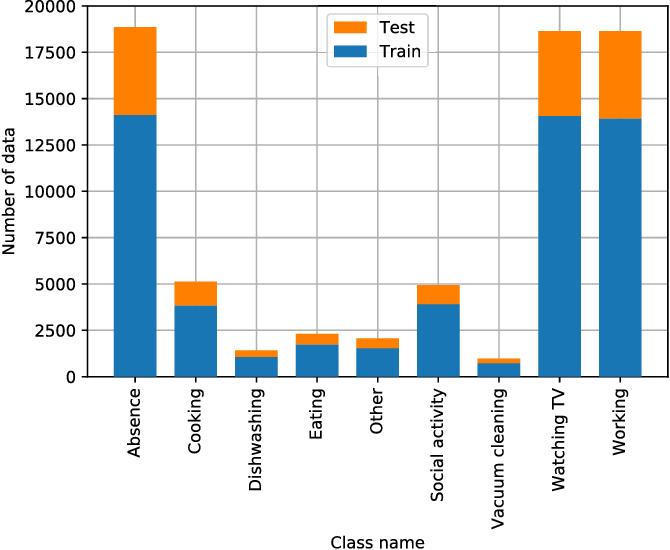
\includegraphics[scale=0.35]{baa-documentation/img/DCASE_unbalanced.png}
	\caption[Data distribution of each activity in Fold 1 of the development dataset]{Data distribution of each activity in Fold 1 of the development dataset \footnotemark}
	\label{fig:DCASE-Unbalanced}
\end{figure}
\footnotetext{\fullcite{inoue_domestic_2018}}
\noindent
\newline
\newline
The augmentation of the audio data is based on two assumptions. First, it is assumed that the acoustic environment does not depend on the order of sound events. For example, consider a recorded audio file within the class \textit{eating}. Some of the sounds correspond to the sound of events made by kitchen utensils and some to the process of eating. Even if the order of these sound events is swapped, the new sound can still be categorised as \textit{eating}. Therefore new data can be generated by changing the order of sound events. The second assumption is that mixing two sounds in the same class generates new sound within the same class. This assumption has also been used in previous works and has proven to be a beneficial data augmentation technique for audio.\footnote{\fullcite{zhang_mixup_2018}}\footnote{\fullcite{takahashi_deep_2016}}
\newline
\newline
For the \fullref{sub:Music-Dataset}, the data augmentation was neglected because the dataset is not imbalanced and extensive enough. There are precisely 30 songs in each class which indicates a relatively equally distributed dataset.
\begin{figure}[htbp]
	\centering
	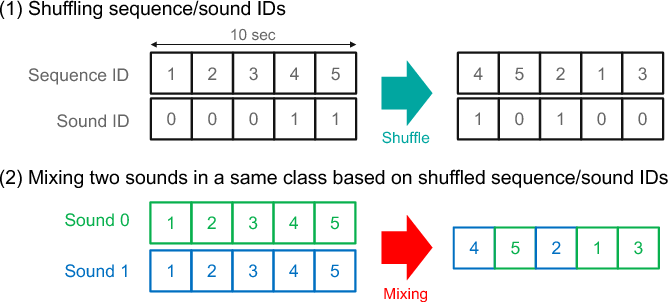
\includegraphics[scale=0.5]{baa-documentation/img/DCASE_data_augmentation.png}
	\caption[Generating new data based on shuffling and mixing]{Generating new data based on shuffling and mixing \footnotemark}
	\label{fig:DCASE-Data-Augmentation}
\end{figure}
\footnotetext{\fullcite{inoue_domestic_2018}}

\section{Triplet selection}
\label{sec:Triplet-Selection}
The triplet selection describes the process of selecting a neighbouring and opposite feature from a given anchor feature. It is described in further detail within section \fullref{eq:Triplet-Loss}. The procedure is split into two parts, the selection of the neighbouring and opposite tile.
\newline
\newline
The straightforward way to triplet selection, as described in \ref{eq:Triplet-Loss} is to select the anchor and the neighbour to be part of the same label and to select the neighbour to have a different label than the other. This approach can not be used in an unsupervised learning technique because the data does not have any information about the underlying label. Due to that, a different, unsupervised approach to triplet selection has to be chosen.
\newline
\newline
For the triplet selection of the \fullref{sub:DCASE-Task-Dataset}, all of the 10s audio files first have to be split into a specified sample length (e.g. 1s, 2s). This results in different segments of the same audio file, which are referred to as segments. The sample length specifies the audio length of all the segments. Therefore a triplet consists of three different segments.
\newline
For the anchor tile, a random segment is chosen. For the neighbouring tile, a segment will be selected which belongs to the same audio file as the anchor. The selection has to be within a predefined range, neighbouring selection range (e.g. 2s, 4s), of the anchor tile. It is important to note, that it does not make any difference if the tile is being sampled from before or after the anchor segment. The opposite tile will be chosen at random from a different audio sample, where the selection of the segment is also performed at random. The only constraint is that the opposite tile can not be chosen from the same audio file as the anchor and the neighbour.
\newline
\newline
For the \fullref{sub:Music-Dataset}, the triplet selection is made relatively similar to the one described in the paragraph above for the \fullref{sub:DCASE-Task-Dataset}. The only difference between the two methods is, that for the \nameref{sub:Music-Dataset} the audio files are of variable length. However, this does not make any difference in the selection algorithm. The sample length and neighbouring selection range will be increased due to the increased audio file length.

\section{Input pipeline}
\label{sec:Input-Pipeline}
The input pipeline is responsible for creating the dataset, which will then be fed into the model by batches. For this project, the input pipeline is implemented using the Tensorflow \texttt{tf.data} API\footnotemark, along with a generator, which loops over the whole dataset and creates entries on the fly. A generator function is used because the entire dataset can not be loaded into memory, due to the large size of it.
\footnotetext{\url{https://www.tensorflow.org/api_docs/python/tf/data}}
\newline
\newline
Because no preprocessing is being done to the datasets and they are used as-is, the input pipeline will need to do the \fullref{sec:Feature-Extraction}, the \fullref{sec:Data-Augmentation} and the \fullref{sec:Triplet-Selection}.
\newline
First, the input pipeline has to generate the dataset using the generator function of the corresponding dataset, which also includes the triplet selection. It is important to note that all the operations after are done on the whole batch. After the generation, the data augmentation, if needed, and then the feature extraction is being performed.
\newline
\newline
The generator function loops over the whole dataset and creates an audio triplet, which will then be yielded back to the dataset. The first step in the generator is the triplet selection. It returns a triplet consisting of the audio file index and the index of the segment within the audio, for the anchor, neighbour and opposite tile. Then these indices will then be used to extract the specified segment of the audio files. Finally, these audio triplet slices will then be yielded back to the dataset from the generator.
\newline
\newline
This creates the dataset dynamically because the dataset only contains the current batch along with some prefetched entries, which are entries from the next batch so that the \gls{GPU} is fully utilised.
\newline
\newline
The feature extraction is implemented using the vectorised \texttt{.map} function of the class \texttt{tf.data.Dataset}\footnotemark. The \texttt{.map} function applies a given function to each element within the dataset, which in our case will be used to extract the features from the audio. Hence a \flqq feature extractor\frqq \ has to be provided to the input pipeline, which will extract a certain feature from the audio as stated in \fullref{sec:Feature-Extraction}.
\footnotetext{\url{https://www.tensorflow.org/api_docs/python/tf/data/Dataset}}
% TODO insert illustration of process

\section{Models}
\label{sec:Models}
This section describes the overall architecture of the models used in the thesis. Audio data will be thought of as two-dimensional data, and therefore state-of-the-art image recognition models can also be used for the audio domain.
\newline
\newline
One of the most straight forward architectures used, are \fullref{sub:Convolutional-Neural-Network}. They are used in a lot of audio applications because of their simplicity and robustness. A lot of research in the past couple of years has shown the overall success of these models.
\newline
\newline
Another widely used model architecture is the \gls{RNN}, such as \fullref{sub:Gated-Recurrent-Unit}, which are primarily used in the text domain. They have also shown their success within the audio domain, because of the sequential nature of the data.
\newline
\newline
The most prominent approach in audio research is the combination of \gls{CNN} and \gls{RNN}. The architecture consists of multiple convolution layers and then single or multiple recurrent layers. These models first reduce the input data to a specific lower-dimensional representation and then use recurrent models to make use of the sequential nature of the data. Therefore the best ideas of both models are used within these \gls{CRNN}.

\section{Application to music}
\label{sec:Application-Music}
All of the concepts mentioned above are designed to work with both datasets. Thus the application to music is described in each above section separately when the application for the \fullref{sub:Music-Dataset} is described.
